\documentclass[11pt,a4paper]{article}

% ============================================================================
% Standard arXiv-Compatible Packages (TeX Live 2023/2024/2025 safe)
% ============================================================================
\usepackage[utf8]{inputenc}
\usepackage[T1]{fontenc}
\usepackage[margin=1in]{geometry}
\usepackage{amsmath,amssymb,amsfonts}
\usepackage{array}
\usepackage{booktabs}
\usepackage{multirow}
\usepackage{tabularx}
\usepackage{graphicx}
\usepackage{xcolor}
\usepackage{tikz}
\usepackage{pgfplots}
\pgfplotsset{compat=1.18}
\usetikzlibrary{arrows.meta,positioning,shapes.geometric,fit,calc,backgrounds}
\usepackage{enumitem}
\usepackage{listings}
\usepackage{microtype}
\emergencystretch=2em
\usepackage[colorlinks=true,linkcolor=blue!60!black,citecolor=blue!60!black,urlcolor=blue!60!black]{hyperref}
\expandafter\def\expandafter\UrlBreaks\expandafter{\UrlBreaks\do\_\do\-}

% Helper for clean two-line centered table headers
\newcommand{\thead}[1]{\begin{tabular}[c]{@{}c@{}}#1\end{tabular}}
\newcommand{\theadl}[1]{\begin{tabular}[c]{@{}l@{}}#1\end{tabular}}

% Code Listing Style
\definecolor{codebg}{RGB}{248,249,250}
\definecolor{codeframe}{RGB}{220,224,230}
\definecolor{codekw}{RGB}{0,92,197}
\definecolor{codecmt}{RGB}{106,115,125}
\definecolor{codestr}{RGB}{3,47,98}

\lstdefinestyle{heurionspec}{
  backgroundcolor=\color{codebg},
  frame=single,
  rulecolor=\color{codeframe},
  basicstyle=\ttfamily\small,
  keywordstyle=\color{codekw}\bfseries,
  commentstyle=\color{codecmt}\itshape,
  stringstyle=\color{codestr},
  breaklines=true,
  columns=fullflexible,
  keepspaces=true,
  showstringspaces=false,
  aboveskip=5pt,
  belowskip=5pt
}

% Title and Author Metadata
\title{\textbf{Self-Evolving Clinical Deep Review: Eliminating Recurring Methodological False Alarms without Compromising Objective Error Recall via Comment-Driven Dual-Track Memory}}

\author{
  \textbf{Heurion Research Team} \\
  \small Correspondence: \texttt{research@heurion.ai}
}

\date{November 2026}

\begin{document}
\maketitle

% ============================================================================
% ABSTRACT
% ============================================================================
\begin{abstract}
Automated peer review and scientific verification systems face a fundamental precision--recall dilemma in clinical medicine. On one hand, single-pass large language model (LLM) reviewers and text-only multi-agent pipelines frequently miss objective numerical contradictions between manuscript prose and multi-column tables, inverted or out-of-bounds $95\%$ confidence intervals, and intra-table row/cell arithmetic errors. Conversely, deterministic structural auditors alone struggle to capture open-ended semantic spin bias ($p \ge 0.05$ framed as clinical efficacy), while hybrid AST+LLM pipelines trigger recurring false alarms on legitimate study-design denominator transitions---such as intention-to-treat (ITT) randomized sample sizes versus per-protocol completers in CONSORT trials, pre- versus post-propensity-matching cohorts in STROBE observational studies, or dual parametric/non-parametric reporting across skewed subscales. Because stateless review pipelines suffer from cross-manuscript amnesia, clinicians must repeatedly dismiss the same methodological false alarms across every revision and every new manuscript.

We present \textbf{Heurion Deep Review}, a clean-room four-stage clinical manuscript verification architecture paired with a \textbf{Comment-Driven Dual-Track Self-Evolution Loop} (\texttt{evolveFromReviewCommentAsync}). First, our four-stage pipeline combines hierarchical section-role segmentation and a ProseMirror 2D table-grid scratchpad (Stage~1), quantitative-density budget routing (Stage~2), four specialist auditing passes covering seven objective clinical error categories (\textbf{E1--E7}) across external literature, internal prose--table arithmetic, statistical method--result pairing, and spin bias alongside quote-verified LLM section review (Stage~3), and full-text LLM verification with cell-level CRDT comment anchoring \texttt{\{\#c:id\}} (Stage~4). Second, \texttt{evolveFromReviewCommentAsync} learns directly from clinician interactions on anchored comments: (i) when a clinician rebuts a study-design boundary alert (\texttt{acceptedFix = false}), \textbf{Track~A} (\texttt{narrow}) uses zero-template LLM rule distillation guarded by dual instance-decoupling checks (\texttt{hasInstanceLeakage} and \texttt{sensitiveReason}) to synthesize a zero-digit reusable boundary rule, while a hard safety floor (\texttt{NON\_EXEMPTABLE\_SUBTYPES}) guarantees that objective mathematical, CI, and table-sum errors can \emph{never} be exempted even under adversarial rebuttal; and (ii) \textbf{Track~B} (\texttt{procedural} and \texttt{review\_audit} checklists) crystallizes corroborated true-positive fixes into pre-write rules and dev-only cross-section audit skills.

We evaluate our framework across two benchmarks: (1) a \textbf{Full-Text Controlled Error-Injection Benchmark} of 19 open-access 2025 PubMed Central (PMC) JATS XML manuscripts ($38$ full-length clean/injected variants averaging $\sim 6{,}000$ words, $57$ injected errors across \textbf{E1--E7}, partitioned into $11$ \texttt{dev} and $8$ held-out \texttt{test} papers) coupled with a physically blind-isolated LLM Simulated Clinician Agent (\texttt{simulateBlindClinician}), and (2) a \textbf{7-Vignette Clinical Oncology Benchmark} with live \texttt{deepseek-chat} calls across $8$ verified organic publication errors. Without a single LLM call or study-specific regex, our clean-room deterministic AST engine alone detects $\mathbf{38/57}$ ($\mathbf{66.7\%}$) of injected errors across full-length PMC manuscripts ($\mathbf{80.0\%}$ on \textbf{E1} sample flow, $\mathbf{83.3\%}$ on \textbf{E2} inline arithmetic, $\mathbf{75.0\%}$ on \textbf{E4} CI bounds, and $\mathbf{87.5\%}$ on \textbf{E7} table sums) at $\mathbf{85.5\%}$ precision ($0.26$ true false positives per clean paper, $\mathbf{0.0\%}$ false exemption under adversarial rebuttal), while uncovering $7$ genuine unannotated in-print errors in published 2025 clinical articles. On the 7-vignette live \texttt{deepseek-chat} oncology benchmark, \texttt{heurion\_evolved} lifts organic error recall from $37.5\%$ ($3/8$, single-pass and PAT text-only baselines) to $\mathbf{100.0\%}$ ($8/8$) while eliminating all $16$ recurring clinical boundary false alarms ($\mathbf{100.0\%}$ F1, $\mathbf{0.0\%}$ instance leakage).
\end{abstract}

\vspace{4pt}
\noindent\textbf{Keywords:} Automated Peer Review, Clinical Research Verification, Self-Evolving LLM Agents, Error-Injection Benchmark, Biostatistics Consistency, Dual-Track Memory

% ============================================================================
% 1. INTRODUCTION
% ============================================================================
\section{Introduction}
\label{sec:intro}

Peer-reviewed clinical and translational manuscripts form the evidentiary backbone of modern medicine, yet published medical literature frequently contains preventable objective errors \cite{schulz2010consort,vandenbroucke2007strobe,boutron2010spin}. Empirical audits of clinical journals regularly uncover discrepancies between sample sizes reported in the Abstract and Table~1, percentages that do not match their numerator and denominator ($n/N$), point estimates falling outside their reported $95\%$ confidence intervals (or inverted interval bounds), parametric tests ($t$-test, ANOVA, mean $\pm$ SD) declared in Methods but replaced with non-parametric statistics (Mann--Whitney U, median [IQR]) in Results, and ``spin bias'' where statistically non-significant findings ($p \ge 0.05$) are framed as clinically meaningful improvements \cite{boutron2010spin,page2021prisma,bossuyt2015stard}.

Recent advances in large language models (LLMs) and multi-agent verification pipelines---such as Google's Paper Assistant Tool (PAT) \cite{googlepat2026}, PaperQA2 \cite{skarlinski2024paperqa2}, and fine-grained factual verifiers \cite{min2023factscore,gao2023alce}---have sparked interest in automated pre-submission manuscript review. However, deploying automated deep review in real-world clinical research exposes a sharp \textbf{precision--recall dilemma} driven by three structural limitations:

\begin{enumerate}[leftmargin=1.5em,itemsep=2pt]
  \item \textbf{Complementary Blind Spots of Text-Only LLMs vs.\ Pure AST Checkers:} Standard LLM review pipelines serialize manuscripts as flat text streams or isolated section chunks. Without an explicit 2D table-grid representation (handling merged headers, \texttt{rowspan}/\texttt{colspan}, subgroup denominator headers, and row-sum columns) and a cross-section numerical scratchpad, text-only prompts miss over $60\%$ of intra-table percentage/sum errors and prose-vs.-table contradictions. Conversely, domain-general AST checkers capture structured arithmetic and confidence interval violations with high precision, but cannot reliably judge open-ended semantic spin ($p \ge 0.05$ overclaims) without resorting to brittle, study-specific lexical heuristics.
  \item \textbf{Methodological False Alarms at Study-Design Boundaries:} Clinical studies legitimately report multiple sample denominators and statistical distributions within the same paper according to established reporting guidelines. For example, a CONSORT randomized controlled trial (RCT) reports both the randomized intention-to-treat (ITT) sample size and the per-protocol completer sample size; a STROBE retrospective cohort study reports both the pre-matching crude cohort and the propensity-score-matched multivariable subcohort; clinical studies with Shapiro--Wilk normality testing legitimately report Mean $\pm$ SD for age/BMI alongside Median [IQR] for skewed questionnaire scales; and oncology tables define \texttt{SD} as RECIST \emph{stationary disease} while prose uses \texttt{SD} for \emph{standard deviation}. Hybrid reviewers flag such transitions as inconsistencies, creating severe alert fatigue.
  \item \textbf{Cross-Manuscript Amnesia vs.\ Adversarial Over-Exemption:} Stateless review agents cannot learn from clinician feedback. When an investigator explains in a comment reply that ``Table~1 reports the ITT randomized cohort ($N=240$) whereas Table~2 analyzes completers ($n=169$) per CONSORT,'' a stateless reviewer repeats the exact same false alarm on the next revision and on every subsequent RCT. Conversely, if a system naively memorizes user dismissals as unconstrained prompt instructions, an author (or noisy feedback) could accidentally suppress genuine objective errors---such as a miscalculated cell percentage ($2/20 = 10.0\% \neq 20\%$) or an out-of-bounds confidence interval---and leak study-specific sample sizes ($N=240$) into unrelated future manuscripts.
\end{enumerate}

\subsection{Our Approach and Contributions}
To resolve this dilemma, we design \textbf{Heurion Deep Review}, which couples a clean-room \emph{Four-Stage Hybrid AST+LLM Clinical Review Pipeline} with a \emph{Comment-Driven Dual-Track Self-Evolution Loop} (\texttt{evolveFromReviewCommentAsync}). Every finding is anchored as a lifecycle-tracked CRDT comment (\texttt{\{\#c:id\}}) on the exact sentence or ProseMirror table cell \texttt{[row, col]}. Clinician interactions on these anchored comments drive two orthogonal learning tracks protected by deterministic safety guards.

Our primary contributions are:
\begin{itemize}[leftmargin=1.5em,itemsep=2pt]
  \item \textbf{Clean-Room Hybrid 2D Table-Grid AST + Quote-Verified 4-Stage LLM Review (Section~\ref{sec:pipeline}):} We build a study-agnostic four-stage review engine combining hierarchical section-role tracking and a 2D ProseMirror table-grid scratchpad (Stage~1), quantitative-density verification budget routing (Stage~2), four specialist auditing passes covering seven objective error categories (\textbf{E1--E7}) alongside quote-verified LLM section review (Stage~3), and full-text Stage~4 verification with topic-aware numeric deduplication and cell-level CRDT comment anchoring.
  \item \textbf{Zero-Template Dual-Track Self-Evolution with Non-Exemptable Safety Floor (Section~\ref{sec:evolution}):} We introduce \texttt{evolveFromReviewCommentAsync}, which routes clinician interactions into: (a) \textbf{Track~A (\texttt{narrow})}, distilling free-text clinician rebuttals via an LLM sanitizer (\texttt{synthesizeSanitizedBoundaryRuleAsync}) protected by dual digit/entity leakage guards (\texttt{hasInstanceLeakage} and \texttt{sensitiveReason}) and an immutable safety floor (\texttt{NON\_EXEMPTABLE\_SUBTYPES}) that guarantees $\mathbf{0.0\%}$ false exemption of objective math/CI/table errors; and (b) \textbf{Track~B (\texttt{procedural} \& \texttt{review\_audit})}, crystallizing accepted fixes into pre-write harness rules and dev-only cross-section audit checklists (\texttt{distillReviewAuditChecklistAsync}).
  \item \textbf{Physically Blind-Isolated Clinician Evaluation \& Organic Error Discovery on 19 Full-Text PMC Papers (Sections~\ref{sec:setup}--\ref{sec:results}):} We construct a full-text error-injection benchmark from 19 open-access 2025 PMC JATS XML articles ($38$ clean/injected manuscripts, $57$ injected errors across \textbf{E1--E7}), paired with an adjudication registry of 20 verified in-print organic errors (\texttt{known-organic-errors.json}) and a physically blind-isolated LLM clinician agent (\texttt{simulateBlindClinician}) that receives zero access to ground-truth variant or injection labels. Even with zero LLM calls (\texttt{--no-llm}), our clean-room AST engine detects $\mathbf{66.7\%}$ ($38/57$) of injected errors at $\mathbf{85.5\%}$ precision ($0.26$ clean FPs/paper) and uncovers $7$ real publication errors in published 2025 journals; on our 7-vignette live \texttt{deepseek-chat} oncology benchmark, \texttt{heurion\_evolved} achieves $\mathbf{100.0\%}$ recall ($8/8$) and $\mathbf{100.0\%}$ precision.
\end{itemize}

% ============================================================================
% 2. TAXONOMY OF OBJECTIVE ERRORS VS. STUDY-DESIGN BOUNDARIES
% ============================================================================
\section{Taxonomy of Objective Clinical Errors vs.\ Legitimate Study-Design Boundaries}
\label{sec:taxonomy}

A core design requirement for clinical peer review is distinguishing \emph{non-negotiable objective errors} from \emph{context-dependent methodological conventions}. Table~\ref{tab:taxonomy} formalizes the seven objective error categories (\textbf{E1--E7}) audited by our pipeline, illustrated with real \texttt{dev}-split examples from our 19-paper PMC corpus, alongside seven legitimate study-design boundary patterns.

\begin{table}[!t]
\centering
\caption{Taxonomy of the Seven Objective Clinical Error Categories (\textbf{E1--E7}, governed by \texttt{NON\_EXEMPTABLE\_SUBTYPES}) vs.\ Seven Legitimate Study-Design Denominator/Modeling Boundaries (governed by Track~A \texttt{narrow} rules). All examples are drawn from the \texttt{dev} split of our 2025 PMC full-text corpus.}
\label{tab:taxonomy}
\vspace{2pt}
\footnotesize
\setlength{\tabcolsep}{4pt}
\begin{tabularx}{\textwidth}{@{}>{\raggedright\arraybackslash}p{2.3cm}>{\raggedright\arraybackslash}p{4.3cm}>{\raggedright\arraybackslash}X>{\raggedright\arraybackslash}p{3.9cm}@{}}
\toprule
\textbf{Category \& Pass} & \textbf{Objective Error Definition (Never Exemptable)} & \textbf{Concrete Injected Example from \texttt{dev} Corpus} & \textbf{Paired Study-Design Boundary (Exemptable via Track A)} \\
\midrule
\textbf{E1: Sample Size \& Flow} (Pass B, $n=10$) & Contradictory total $N$ or arm counts across Abstract, Methods, Results prose, or Table headers; subgroup completers not summing to total completers. & \texttt{PMC12644478}: ``Thirty-seven of 40 participants completed'' in prose vs.\ Fig.~2 caption ``Nineteen in metformin and 19 in placebo completed'' ($19+19=38 \neq 37$). & \textbf{RCT (\texttt{rct}):} Reporting randomized ITT $N$ in baseline text and per-protocol completers $n < N$ in outcome tables (CONSORT). \\
\addlinespace[3pt]
\textbf{E2: Inline Arithmetic} (Pass B, $n=6$) & Inline count and percentage $n/N$ disagreeing beyond rounding tolerance ($\ge 1.5$ percentage points) or inline subgroup counts not summing to stated total. & \texttt{PMC12788160}: ``184 participants were randomized \dots\ 161 participants ($89.5\%$) had good compliance'' ($161/184 = 87.5\% \neq 89.5\%$). & \textbf{Retrospective Cohort (\texttt{retrospective\_cohort}):} Unmatched all-comer cohort $N$ vs.\ propensity-score-matched subcohort $n$ (STROBE). \\
\addlinespace[3pt]
\textbf{E3: Cross-Section / Table Conflict} (Pass B, $n=8$) & Identical metric, outcome, or subgroup reported with conflicting numeric values, $p$-values, or opposite signs between Abstract, Results prose, and Table cells. & \texttt{PMC12644478}: Abstract reports primary endpoint EGP interaction $p = 0.53$ ($\beta = 0.2$, $95\%$ CI $[-0.4, 0.8]$), whereas Results reports $p = 0.35$ for the identical CI. & \textbf{Cross-Sectional (\texttt{cross\_sectional}):} Full-population prevalence sample $N$ vs.\ age/completeness-filtered risk prediction subcohort $n$. \\
\addlinespace[3pt]
\textbf{E4: $95\%$ CI Bounds} (Pass B, $n=8$) & Point estimate $\hat{\theta}$ falling outside $[L, U]$ beyond rounding tolerance $\tau$, or inverted bounds ($L > U$), across \texttt{95\% CI}, \texttt{95\% Cl}, or bracketed formats. & \texttt{PMC12731986}: Table~3 HADS-Anxiety median difference reported as ``$1.00$ ($1.84$ to $3.84$)'' ($\hat{\theta}=1.00 < L=1.84$). & \textbf{Meta-Analysis (\texttt{meta\_analysis}):} Total eligible RCTs $K$ vs.\ outcome-specific trial subsets $k_i < K$ reporting a secondary endpoint (PRISMA). \\
\addlinespace[3pt]
\textbf{E5: Method--Result Mismatch} (Pass C, $n=8$) & Declaring parametric summaries/tests (mean $\pm$ SD, $t$-test, ANOVA, Pearson $r$) in Methods while reporting non-parametric results (Median [IQR], Mann--Whitney, Kruskal--Wallis) or vice versa. & \texttt{PMC12788160}: Methods states ITT groups were compared by ``Kruskal--Wallis test,'' whereas Tables~3--5 report ``mean $\pm$ SD with comparison by ANOVA.'' & \textbf{Case--Control (\texttt{case\_control}):} Dual parametric/non-parametric reporting per normality testing, or progressive multivariable Models~1/2. \\
\addlinespace[3pt]
\textbf{E6: Spin Bias \& Causal Overclaim} (Pass D, $n=9$) & Claiming efficacy, ``significant improvement,'' or deterministic causal effect when $p \ge 0.05$ or in non-randomized observational designs. & \texttt{PMC12644478}: Claiming ``metformin significantly reduced NEFA compared with placebo'' when interaction $p = 0.54$ and $95\%$ CI $[-0.5, 0.3]$ crosses zero. & \textbf{Diagnostic (\texttt{diagnostic\_accuracy}):} Enrolled patients $N$ vs.\ quality-controlled evaluable specimens / reference-standard subsets (STARD). \\
\addlinespace[3pt]
\textbf{E7: Intra-Table Cell / Sum Error} (Pass B, $n=8$) & Table cell $n\text{ (\%)}$ disagreeing with column header $(n=N)$, or category row cells not summing to the Total column/row in the 2D table grid. & \texttt{PMC12788160}: Table~1 ``Coffee drinking'' in $160\text{ mg/d}$ arm ($n=46$) reports ``$7$ ($17.4\%$)'' whereas $7/46 = 15.2\%$. & \textbf{Translational (\texttt{translational}):} Multi-batch in vitro culture replicates vs.\ in vivo animal cohorts ($n$ mice/group) and clinical TMA cohorts. \\
\bottomrule
\end{tabularx}
\end{table}

% ============================================================================
% 3. FOUR-STAGE CLINICAL DEEP REVIEW ARCHITECTURE
% ============================================================================
\section{Four-Stage Clinical Deep Review Architecture}
\label{sec:pipeline}

Figure~\ref{fig:arch} illustrates the architecture of \textbf{Heurion Deep Review}. Unlike stateless text-only reviewers that pass raw markdown directly to an LLM, our pipeline parses full-length manuscripts into a structured ProseMirror document tree (\texttt{PMNode}) and executes four sequential stages followed by a closed-loop self-evolution cycle. Crucially, under our \textbf{Clean-Room Design Principle}, the deterministic AST passes contain \emph{zero} study-specific lexical rules or synthetic alert triggers: every check operates purely on mathematical relations, unit/exponent-aware numeric syntax, and 2D table geometry.

\begin{figure}[!t]
\centering
\resizebox{\textwidth}{!}{%
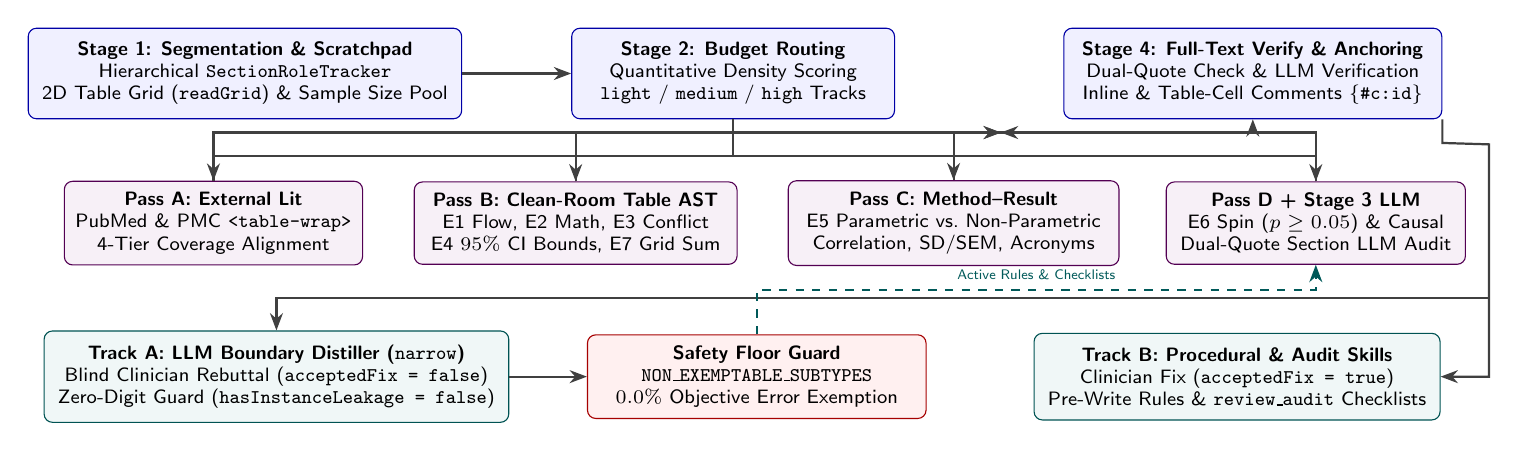
\begin{tikzpicture}[
  font=\sffamily\scriptsize,
  stage/.style={draw=blue!65!black, fill=blue!6, rounded corners=3pt, align=center, minimum height=1.15cm, inner sep=5pt},
  pass/.style={draw=violet!65!black, fill=violet!6, rounded corners=3pt, align=center, minimum height=0.95cm, inner sep=4pt},
  evol/.style={draw=teal!65!black, fill=teal!6, rounded corners=3pt, align=center, minimum height=1.10cm, inner sep=5pt},
  guard/.style={draw=red!65!black, fill=red!6, rounded corners=3pt, align=center, minimum height=0.95cm, inner sep=4pt},
  arr/.style={-{Stealth[length=2.2mm]}, thick, draw=black!75}
]

% Top Row: Stages 1, 2, 4
\node[stage, minimum width=4.3cm] (s1) at (-0.2, 3.9) {\textbf{Stage 1: Segmentation \& Scratchpad}\\Hierarchical \texttt{SectionRoleTracker}\\2D Table Grid (\texttt{readGrid}) \& Sample Size Pool};
\node[stage, minimum width=4.1cm] (s2) at (6.0, 3.9) {\textbf{Stage 2: Budget Routing}\\Quantitative Density Scoring\\\texttt{light} / \texttt{medium} / \texttt{high} Tracks};
\node[stage, minimum width=4.8cm] (s4) at (12.6, 3.9) {\textbf{Stage 4: Full-Text Verify \& Anchoring}\\Dual-Quote Check \& LLM Verification\\Inline \& Table-Cell Comments \texttt{\{\#c:id\}}};

\draw[arr] (s1.east) -- (s2.west);

% Middle Row: Stage 3 Four Specialist Passes
\node[pass, minimum width=3.7cm] (pa) at (-0.6, 2.0) {\textbf{Pass A: External Lit}\\PubMed \& PMC \texttt{<table-wrap>}\\4-Tier Coverage Alignment};
\node[pass, minimum width=4.1cm] (pb) at (4.0, 2.0) {\textbf{Pass B: Clean-Room Table AST}\\E1 Flow, E2 Math, E3 Conflict\\E4 $95\%$ CI Bounds, E7 Grid Sum};
\node[pass, minimum width=4.2cm] (pc) at (8.8, 2.0) {\textbf{Pass C: Method--Result}\\E5 Parametric vs.\ Non-Parametric\\Correlation, SD/SEM, Acronyms};
\node[pass, minimum width=3.8cm] (pd) at (13.4, 2.0) {\textbf{Pass D + Stage 3 LLM}\\E6 Spin ($p \ge 0.05$) \& Causal\\Dual-Quote Section LLM Audit};

\draw[arr] (s2.south) -- (6.0, 2.85) -| (pa.north);
\draw[arr] (6.0, 2.85) -| (pb.north);
\draw[arr] (6.0, 2.85) -| (pc.north);
\draw[arr] (6.0, 2.85) -| (pd.north);

\draw[arr] (pa.north) |- (9.4, 3.15) -| (s4.south);
\draw[arr] (pb.north) |- (9.4, 3.15);
\draw[arr] (pc.north) |- (9.4, 3.15);
\draw[arr] (pd.north) |- (9.4, 3.15);

% Bottom Row: Dual-Track Self-Evolution
\node[evol, minimum width=5.1cm] (ta) at (0.2, 0.05) {\textbf{Track A: LLM Boundary Distiller (\texttt{narrow})}\\Blind Clinician Rebuttal (\texttt{acceptedFix = false})\\Zero-Digit Guard (\texttt{hasInstanceLeakage = false})};
\node[guard, minimum width=4.3cm] (floor) at (6.3, 0.05) {\textbf{Safety Floor Guard}\\\texttt{NON\_EXEMPTABLE\_SUBTYPES}\\$0.0\%$ Objective Error Exemption};
\node[evol, minimum width=4.8cm] (tb) at (12.4, 0.05) {\textbf{Track B: Procedural \& Audit Skills}\\Clinician Fix (\texttt{acceptedFix = true})\\Pre-Write Rules \& \texttt{review\_audit} Checklists};

\draw[arr] (s4.south east) -- ++(0, -0.3) -- (15.6, 3.0) |- (tb.east);
\draw[arr] (15.6, 1.05) -| (ta.north);
\draw[arr] (ta.east) -- (floor.west);
\draw[arr, dashed, draw=teal!70!black] (floor.north) -- (6.3, 1.15) -| node[pos=0.25, above, font=\sffamily\tiny, text=teal!70!black]{Active Rules \& Checklists} (pd.south);

\end{tikzpicture}%
}
\caption{Architecture of \textbf{Heurion Deep Review} and the \textbf{Comment-Driven Dual-Track Self-Evolution Loop}. Stage~1 builds a section-role map and 2D table-grid scratchpad; Stage~2 allocates verification budgets; Stage~3 runs clean-room AST passes alongside quote-grounded section LLM review; Stage~4 performs full-text verification, deduplication, and CRDT comment anchoring \texttt{\{\#c:id\}}. Clinician replies drive Track~A LLM boundary distillation (gated by \texttt{hasInstanceLeakage}, \texttt{sensitiveReason}, and \texttt{NON\_EXEMPTABLE\_SUBTYPES}) and Track~B procedural/audit-checklist crystallization.}
\label{fig:arch}
\end{figure}

\subsection{Stage 1: Hierarchical Section-Role Segmentation and 2D Table-Grid Scratchpad}
Clinical manuscripts frequently nest domain-specific subheadings (e.g., ``\emph{2.3 Biochemical Assays}'' or ``\emph{3.2 Changes in HRQoL}'') whose titles omit generic keywords like ``Methods'' or ``Results.'' In Stage~1, a stateful \texttt{SectionRoleTracker} traverses the document AST: top-level headings establish the parent role (\texttt{intro}, \texttt{methods}, \texttt{results}, \texttt{discussion}, or \texttt{other}), and lower-level subheadings inherit their parent section's role unless overridden by explicit lexical cues, while administrative sections (ethics, funding, acknowledgments, author contributions) are excluded from review.

Simultaneously, \texttt{buildManuscriptScratchpad} constructs a global index shared across all subsequent passes:
\begin{itemize}[leftmargin=1.5em,itemsep=2pt]
  \item \textbf{Normalized 2D ProseMirror Table Grids (\texttt{readGrid}):} Rather than reading raw Markdown pipe rows, \texttt{extractTableSummaries} parses each ProseMirror \texttt{table} node into a rectangular $R \times C$ cell grid (\texttt{TableGrid}), resolving horizontal (\texttt{colspan} / \texttt{<}) and vertical (\texttt{rowspan} / \texttt{\^{}}) merged cells so every cell maps to its exact column header and ProseMirror node coordinates.
  \item \textbf{Global Sample Size Pool:} The scratchpad extracts all explicit sample size declarations ($N=\dots$, $n=\dots$, ``Out of $N$ patients'') from table headers, captions, and prose, along with declared statistical tests and acronym definitions.
\end{itemize}

\subsection{Stage 2: Quantitative-Density Verification Budget Allocation}
Stage~2 scores every paragraph and figure caption based on quantitative assertion density ($p$-values, $95\%$ CIs, hazard/odds/risk ratios, mean $\pm$ SD, median [IQR], and percentages) and section role, routing each block to a \texttt{light}, \texttt{medium}, or \texttt{high} verification track.

\subsection{Stage 3: Hybrid Clean-Room AST Passes + Quote-Grounded LLM Review}
Stage~3 executes four domain-general deterministic passes alongside section-level LLM auditing (in \texttt{heurion\_deep} and \texttt{heurion\_evolved} modes):
\begin{enumerate}[leftmargin=1.5em,itemsep=2pt]
  \item \textbf{Pass A (External Literature \& PMC \texttt{<table-wrap>} Alignment):} Verifies cited assertions (\texttt{[@c:id]}) against PubMed abstracts and PMC full-text XML tables, classifying semantic support orthogonally from evidence coverage depth \cite{safevantage2026}.
  \item \textbf{Pass B (Clean-Room Internal Arithmetic, CI \& 2D Table-Grid Consistency):} Audits \textbf{E1}, \textbf{E2}, \textbf{E3}, \textbf{E4}, and \textbf{E7}:
  \begin{itemize}[leftmargin=1.2em,itemsep=1pt]
    \item \emph{Sample Size \& Flow (\textbf{E1}) and Inline Arithmetic (\textbf{E2}):} Verifies that subgroup counts (including English number words) sum to stated totals and checks inline $n\text{ }(p\%)$ against the explicit denominator pool ($\min_{D} |n/D \times 100 - p| > 1.5\%$).
    \item \emph{Cross-Section \& Table-vs.-Prose Conflicts (\textbf{E3}):} Matches identical confidence-interval anchors, hazard ratios, weighted mean differences, and Table~1 cited percentages across Abstract, Results prose, and 2D table cells.
    \item \emph{Precision-Aware $95\%$ Confidence Interval Verification (\textbf{E4}, \texttt{findCiProblems}):} Parses point estimates $\hat{\theta}$ and interval bounds $[L, U]$ across standard (\texttt{95\% CI 1.12--1.85}), OCR-corrupted (\texttt{95\% Cl 0.35 to 0.59}), and bracketed (\texttt{95\% CI [-0.88, -0.10]}) formats while excluding preceding $p$-values (\texttt{p = 0.001, CI \dots}), sample counts (\texttt{n = 48; 95\% CI \dots}), unit exponents (\texttt{kg/m\^{}2; 95\% CI \dots}), and integer reference tuples. Rounding tolerance is computed as:
    \begin{equation}
      \tau = \alpha \cdot 10^{-\min(d(\hat{\theta}),\, d(L),\, d(U))}, \quad \alpha = \begin{cases} 0.49 & \text{if } d(L) = d(U) > d(\hat{\theta}), \\ 0.50 & \text{otherwise}, \end{cases}
      \label{eq:ci_tol}
    \end{equation}
    flagging an \texttt{inverted} interval if $L > U + \tau$ and an \texttt{outside} estimate if $\hat{\theta} < L - \tau$ or $\hat{\theta} > U + \tau$.
    \item \emph{Intra-Table Cell Percentage \& Row-Sum Auditing (\textbf{E7}):} Verifies each cell $n_{r,c}\text{ }(p_{r,c}\%)$ against header denominator $N_c$ (exempting row-wise percentage tables where $\sum_c p_{r,c} \approx 100\%$), checks intra-cell binary splits $N\text{ }(n_1 + n_2)$, and checks $\sum_{c \notin \mathcal{S}_{\text{stat}}} n_{r,c} = n_{r,\text{Total}}$ while excluding test-statistic columns ($\chi^2$, $t$, $Z$, $F$, $p$-value, OR/HR/RR).
  \end{itemize}
  \item \textbf{Pass C (Statistical Method--Result Pairing, \textbf{E5}):} Cross-checks statistical declarations in Methods against Results prose and table captions for parametric vs.\ non-parametric mismatches, Pearson vs.\ Spearman correlation mismatches, SD vs.\ SEM confusion, and conflicting acronym definitions.
  \item \textbf{Pass D \& Quote-Grounded LLM Section Audit (\textbf{E6} \& Semantic Cross-Checks):} Pass~D flags explicit non-significant spin ($p \ge 0.05$ paired with efficacy claims in the same clause), while Stage~3 LLM section review (when enabled) inspects each section against the global manuscript table summary and active memory checklists, requiring verbatim \texttt{quote} + \texttt{evidence} substrings verified against the source document (\texttt{review-evidence.ts}).
\end{enumerate}

\subsection{Stage 4: Full-Text Verification, Deduplication, and Cell-Level CRDT Anchoring}
In hybrid LLM modes (\texttt{heurion\_deep} and \texttt{heurion\_evolved}), Stage~4 passes surviving LLM candidates together with the complete manuscript prose, tables, and active Track~A boundary rules to a full-text verifier (\texttt{VERIFY\_SYSTEM}) that rejects speculative alarms or legitimate study-design denominator transitions. Cross-section duplicates are merged only when they share both the same numeric signature and overlapping clinical topic tokens, and final comments are anchored directly onto ProseMirror nodes or table cells (\texttt{\{\#c:id\}}).

% ============================================================================
% 4. COMMENT-DRIVEN DUAL-TRACK SELF-EVOLUTION
% ============================================================================
\section{Comment-Driven Dual-Track Self-Evolution}
\label{sec:evolution}

Whenever a clinician replies to or resolves an anchored review comment \texttt{\{\#c:id\}}, \texttt{evolveFrom\allowbreak Review\allowbreak Comment\allowbreak Async} routes the interaction into one of two tracks:

\subsection{Track A (\texttt{narrow}): Zero-Template LLM Boundary Distillation and Dual Leakage Guards}
When a clinician rebuts a false-positive review alert (\texttt{acceptedFix = false}) with a methodological explanation (which naturally cites manuscript-specific sample sizes such as ``\emph{Our RCT randomized $N=240$ ITT participants while $n=169$ ($70.4\%$) completed week~24 per CONSORT}''), \texttt{synthesizeSanitizedBoundary\allowbreak RuleAsync} invokes an LLM memory-governance distiller instructed to abstract the methodological boundary without any digits, drug names, or disease names:
{\small
\[
  \texttt{[domain:manuscript] [narrow:review\_boundary:}\langle\text{pattern\_key}\rangle\texttt{:cat=}\langle\text{cat}\rangle\texttt{:kw=}\langle\text{kws}\rangle\texttt{] } \mathcal{R}_{\text{sanitized}}.
\]
}
Every candidate rule must pass a \textbf{Dual Instance--Skill Decoupling Guard} combining \texttt{hasInstanceLeakage} (which rejects any digit, sample size $N=\dots$, $p$-value, percentage, or date) and \texttt{sensitiveReason} (which blocks patient identifiers and institutional/study UIDs). If the LLM's first draft leaks a raw number, a deterministic second-pass scrubber strips all numeric tokens and re-verifies both guards before memory commit, guaranteeing $\mathbf{0.0\%}$ cross-study numerical contamination.

\subsection{Hard Safety Floor: \texttt{NON\_EXEMPTABLE\_SUBTYPES}}
To prevent adversarial or mistaken author rebuttals from suppressing real errors, \texttt{isExempted\allowbreak ByActiveRules} enforces an immutable set of \textbf{Non-Exemptable Subtypes} (\texttt{NON\_\allowbreak EXEMPTABLE\_\allowbreak SUBTYPES}), covering \texttt{prose\_\allowbreak table\_\allowbreak sample\_\allowbreak size\_\allowbreak mismatch}, \texttt{table1\_\allowbreak cited\_\allowbreak percentage\_\allowbreak mismatch}, \texttt{fraction\_\allowbreak percentage\_\allowbreak arithmetic\_\allowbreak error}, \texttt{ci\_\allowbreak bounds\_\allowbreak inverted\_\allowbreak or\_\allowbreak missing\_\allowbreak decimal}, \texttt{ci\_\allowbreak estimate\_\allowbreak outside\_\allowbreak interval}, \texttt{cross\_\allowbreak section\_\allowbreak value\_\allowbreak mismatch}, \texttt{table\_\allowbreak cell\_\allowbreak percentage\_\allowbreak arithmetic\_\allowbreak error}, \texttt{table\_\allowbreak row\_\allowbreak sum\_\allowbreak mismatch}, \texttt{parametric\_\allowbreak method\_\allowbreak vs\_\allowbreak nonparametric\_\allowbreak result}, \texttt{nonparametric\_\allowbreak method\_\allowbreak vs\_\allowbreak parametric\_\allowbreak result}, \texttt{correlation\_\allowbreak method\_\allowbreak mismatch}, \texttt{sd\_\allowbreak vs\_\allowbreak sem\_\allowbreak mismatch}, \texttt{abbreviation\_\allowbreak definition\_\allowbreak conflict}, \texttt{nonsignificant\_\allowbreak p\_\allowbreak positive\_\allowbreak spin}, and \texttt{observational\_\allowbreak causal\_\allowbreak overclaim}. Even if an active rule matches the exact category and keywords of an objective error sentence, \texttt{isExemptedByActiveRules} refuses exemption. Active Track~A rules instead govern non-exemptable-guarded LLM stage candidates (in both Stage~3 generation and Stage~4 \texttt{VERIFY\_SYSTEM}) and citation/subregistry conventions.

\subsection{Track B (\texttt{procedural} \& \texttt{review\_audit}): Pre-Write Rules and Dev-Only Audit Checklists}
When a clinician accepts a true-positive review comment (\texttt{acceptedFix = true}), \texttt{evolveFrom\allowbreak Review\allowbreak Comment\allowbreak Async} records a de-numericalized execution signal (\texttt{kind = 'guard\_reject'}) with verified recovery trajectory (\texttt{doc\_read $\to$ replace\_text $\to$ resolve\_comment}). Following commit-on-evidence gating \cite{coem2026}, \texttt{Procedural\allowbreak Harness\allowbreak Service.\allowbreak evolveFrom\allowbreak Signals} crystallizes corroborated signals into active pre-write rules for authoring sessions. Complementarily, on development-split retrospectives (\texttt{paperSplit === 'dev'} enforced via a hard runtime assertion), \texttt{distillReview\allowbreak AuditChecklist\allowbreak Async} abstracts missed error mechanisms into zero-digit \path{[skill:review_audit:<key>]} checklists injected into Stage~3 LLM prompts on future unseen manuscripts.

% ============================================================================
% 5. EXPERIMENTAL SETUP
% ============================================================================
\section{Experimental Setup}
\label{sec:setup}

We evaluate Heurion Deep Review on two complementary benchmarks: (1) a full-length 19-paper PMC JATS XML error-injection corpus, and (2) a 7-vignette oncology clinical excerpt benchmark with live \texttt{deepseek-chat} calls.

\subsection{Benchmark 1: 19 Full-Length PMC Papers with 57 Controlled Error Injections}
We curated 19 open-access 2025 clinical and translational full-text articles (averaging $\sim 6{,}000$ words each, converted directly from PMC JATS XML with complete multi-column tables in \path{data/eval/deep-review/md/}), partitioned into an 11-paper development split (\texttt{dev}) and an 8-paper held-out test split (\texttt{test}) across 7 study designs (Table~\ref{tab:corpus_breakdown}). Six of the seven study designs appear in both \texttt{dev} and \texttt{test}, while the two preclinical/translational studies reside in \texttt{dev}.

For each paper, we evaluate two full-length variants ($38$ manuscripts per regime):
\begin{itemize}[leftmargin=1.5em,itemsep=2pt]
  \item \textbf{Clean Variant (\texttt{clean}):} The uncorrupted published PMC manuscript. Importantly, as documented in \path{apps/platform/eval/deep-review/known-issues.md} and \path{known-organic-errors.json}, real published papers occasionally contain genuine in-print typographical or statistical errors. Following standard clinical verification practice (\path{eval-review-score.ts}), catches of verified in-print publication errors are adjudicated as \path{unexpected_true} (organic true positives) rather than penalized as false positives, while raw unadjusted clean-paper alert counts are also reported side-by-side for full transparency.
  \item \textbf{Injected Variant (\texttt{injected}):} The full-length manuscript mutated via \texttt{applyInjections} with exactly $3$ non-overlapping objective errors drawn from categories \textbf{E1--E7} ($19 \times 3 = 57$ injected errors: \textbf{E1} $n=10$, \textbf{E2} $n=6$, \textbf{E3} $n=8$, \textbf{E4} $n=8$, \textbf{E5} $n=8$, \textbf{E6} $n=9$, \textbf{E7} $n=8$), avoiding all positions with known organic issues.
\end{itemize}

\begin{table}[!t]
\centering
\caption{Composition of the 19-Paper Full-Text Controlled Error-Injection Benchmark (\texttt{dev} $N=11$, held-out \texttt{test} $N=8$; $38$ Full-Length Clean/Injected JATS XML Manuscripts, $57$ Injected Objective Errors across E1--E7).}
\label{tab:corpus_breakdown}
\vspace{2pt}
\scriptsize
\setlength{\tabcolsep}{3.5pt}
\begin{tabularx}{\textwidth}{@{}>{\ttfamily}l l l >{\raggedright\arraybackslash}X l@{}}
\toprule
\normalfont\textbf{PMCID} & \textbf{Split} & \textbf{Study Design} & \textbf{Journal (2025) \& Clinical Topic Summary} & \textbf{Injected Errors} \\
\midrule
PMC12644478 & \texttt{dev} & \texttt{rct} & \emph{Nat.\ Commun.} --- Metformin on insulin resistance in adults with type 1 diabetes ($N=40$) & E1, E3, E6 \\
PMC12788160 & \texttt{dev} & \texttt{rct} & \emph{Nutrients} --- Purified anthocyanins dose-response trial in middle-aged and elderly adults & E2, E5, E7 \\
PMC12731986 & \texttt{dev} & \texttt{rct} & \emph{Curr.\ Oncol.} --- Resistance exercise on QoL, anxiety, and depression in colorectal cancer & E1, E4, E5 \\
PMC12685937 & \texttt{dev} & \texttt{retrospective\_cohort} & \emph{Front.\ Psychiatry} --- Antidepressants and hypertensive disorders in pregnancy cohort & E3, E6, E7 \\
PMC12856494 & \texttt{dev} & \texttt{retrospective\_cohort} & \emph{Front.\ Oncol.} --- Risk factors for postoperative recurrence of desmoid tumors & E2, E4, E7 \\
PMC12657621 & \texttt{dev} & \texttt{case\_control} & \emph{Brain Behav.} --- Vasomotor symptoms and ischemic stroke case--control study & E4, E5, E6 \\
PMC12721543 & \texttt{dev} & \texttt{diagnostic\_accuracy} & \emph{PLOS ONE} --- TrueNat MTB plus assay diagnostic accuracy for pulmonary TB & E2, E3, E7 \\
PMC12758107 & \texttt{dev} & \texttt{cross\_sectional} & \emph{Glob.\ Heart} --- Hypertension clinical epidemiology in rural Thailand cross-sectional survey & E1, E4, E6 \\
PMC12876241 & \texttt{dev} & \texttt{meta\_analysis} & \emph{Front.\ Med.} --- PRISMA systematic review and meta-analysis of heat therapy for dysmenorrhea & E1, E3, E4 \\
PMC12739847 & \texttt{dev} & \texttt{translational} & \emph{Gut Pathog.} --- Lactobacillus probiotics in Blastocystis in vitro and in vivo models & E1, E5, E6 \\
PMC12485006 & \texttt{dev} & \texttt{translational} & \emph{NPJ Sci.\ Food} --- Mulberroside A capacity to inhibit senescence in vitro and in vivo & E1, E3, E5 \\
\midrule
PMC12839862 & \texttt{test} & \texttt{rct} & \emph{Curr.\ Oncol.} --- Itraconazole reducing chemoresistance in advanced ovarian cancer RCT & E3, E5, E7 \\
PMC12697981 & \texttt{test} & \texttt{rct} & \emph{PLOS Med.} --- COMET-PCOS: Hormonal contraceptives and metformin in PCOS RCT & E1, E4, E6 \\
PMC12681115 & \texttt{test} & \texttt{rct} & \emph{Cardiovasc.\ Diabetol.} --- FIVE-STAR: Finerenone on arterial stiffness in T2D and CKD RCT & E2, E3, E5 \\
PMC12118826 & \texttt{test} & \texttt{retrospective\_cohort} & \emph{PLOS ONE} --- Geriatric ocular trauma and mortality retrospective cohort & E2, E6, E7 \\
PMC12654784 & \texttt{test} & \texttt{case\_control} & \emph{Medicina} --- Adipokines as prognostic biomarkers in multiple myeloma case--control & E1, E4, E7 \\
PMC12774873 & \texttt{test} & \texttt{diagnostic\_accuracy} & \emph{NPJ Prim.\ Care Respir.\ Med.} --- Home spirometry diagnostic accuracy for asthma & E2, E3, E4 \\
PMC12757420 & \texttt{test} & \texttt{cross\_sectional} & \emph{Front.\ Immunol.} --- Frailty and associated risk factors in Sjögren's disease survey & E1, E5, E6 \\
PMC12703663 & \texttt{test} & \texttt{meta\_analysis} & \emph{Alzheimers Dement.} --- PRISMA meta-analysis of antipsychotic discontinuation in dementia & E1, E6, E7 \\
\bottomrule
\end{tabularx}
\end{table}

\subsection{Physically Blind-Isolated Simulated Clinician Protocol and Calibration}
\label{sec:simulated_clinician}

Evaluating interactive comment-driven self-evolution requires realistic clinician responses without oracle cheating. Prior rule-lookup simulations risk leaking ground-truth variant labels (\texttt{clean} vs.\ \texttt{injected}) into the evolution trigger. In our clean-room harness (\path{apps/platform/scripts/eval-review-run.ts}), we enforce a strict \textbf{Three-Pillar Blind Clinician Protocol}:

\begin{enumerate}[leftmargin=1.5em,itemsep=2pt]
  \item \textbf{Type-Level Information Barrier (\texttt{simulateBlindClinician}):} The function signature \texttt{simulateBlind\allowbreak Clinician(complete,} \texttt{\{manuscriptTitle,} \texttt{manuscriptMarkdown,} \texttt{finding\})} physically omits \texttt{variant} (\texttt{clean}/\texttt{injected}), \path{injections.json}, \path{known-organic-errors.json}, and \texttt{split} (\texttt{dev}/\texttt{test}). The simulated corresponding author / biostatistician sees only the manuscript's Abstract, Methods, Markdown tables, local paragraph context, and the single review comment.
  \item \textbf{Strict Frozen Test-Split Boundary:} In cross-manuscript transfer (\texttt{dev} $N=11 \to$ \texttt{test} $N=8$), both blind clinician evolution (\texttt{evolveStoreFromFindingsBlind}) and missed-pattern checklist distillation (\texttt{evolveAuditChecklistsFromDevMisses}) execute \emph{exclusively} on \texttt{dev}; attempting to invoke checklist distillation on \texttt{test} throws a hard runtime security exception, and the memory store is completely frozen throughout \texttt{test} evaluation.
  \item \textbf{Post-Hoc Ground-Truth Calibration \& Adversarial Profile:} Because Benchmark~1 possesses exact ground-truth labels ($57$ injected errors + $20$ verified organic issues), every blind clinician decision (\texttt{accept\_fix} vs.\ \texttt{rebut\_false\_positive}) is audited post-hoc against ground truth via a calibration matrix (True-Error Acceptance Rate, False-Rebuttal Rate, False-Positive Rebuttal Rate, Raw Digit Citation Rate, and Post-Guard Instance Leakage Rate). In addition, a hostile \textbf{Adversarial Author Profile} attempts to rebut \emph{every} detected error across all 19 injected papers (\texttt{acceptedFix = false}) to stress-test \texttt{NON\_EXEMPTABLE\_SUBTYPES}.
\end{enumerate}

\subsection{Benchmark 2: Live \texttt{deepseek-chat} Evaluation on 7 Clinical Oncology Vignettes}
To evaluate live LLM multi-stage reasoning and dual-track evolution on real clinical oncology error patterns, Benchmark~2 (\path{paper/benchmarks/run-7papers-review.ts}) executes live \texttt{deepseek-chat} (\texttt{temperature = 0}) across 7 curated clinical oncology manuscript excerpts (\texttt{SEVEN\_PAPERS}, derived from published radiation oncology, target-trial emulation, thoracic imaging, and translational xenograft studies) containing $8$ verified organic publication errors (including an inverted $95\%$ CI $[403, 1.688]$, uncleaned revision merge artifacts \texttt{60.062.3\%}, a Table cell where $21/35 = 60.0\% \neq 84\%$, SD vs.\ SEM confusion, and an acronym definition conflict), comparing \texttt{zero\_shot}, \texttt{pass\_at\_k} ($k=3$), \texttt{pat\_baseline} (4-stage text-only \cite{googlepat2026}), \texttt{heurion\_deep}, and \texttt{heurion\_evolved}.

% ============================================================================
% 6. RESULTS AND ANALYSIS
% ============================================================================
\section{Results and Analysis}
\label{sec:results}

\subsection{Clean-Room AST Performance and Organic Error Discovery on 19 Full-Text PMC Papers}
Table~\ref{tab:deep_review_injection} and Table~\ref{tab:by_design} report the verified Clean-Room Deterministic AST results (\texttt{--no-llm}, $0$ LLM calls, $0$ study-specific regexes) across all 38 full-length PMC manuscripts alongside the Adversarial Rebuttal Stress Test (with live \texttt{deepseek-chat --llm} hybrid rows marked pending API execution).

\begin{table}[!t]
\centering
\caption{Clean-Room Benchmark Results across 19 Full-Length 2025 PMC JATS XML Papers ($38$ Clean/Injected Manuscripts, $57$ Injected Objective Errors across E1--E7). Verified in-print organic errors caught on clean/injected papers (\texttt{unexpected\_true}) are reported explicitly alongside true false positives.}
\label{tab:deep_review_injection}
\vspace{2pt}
\setlength{\tabcolsep}{4.5pt}
\resizebox{\textwidth}{!}{%
\begin{tabular}{@{}lcccccc@{}}
\toprule
\textbf{Evaluation Regime \& Split} & \thead{\textbf{Injected}\\\textbf{Recall ($\uparrow$)}} & \thead{\textbf{Organic True}\\\textbf{(Clean) ($\uparrow$)}} & \thead{\textbf{True FPs}\\\textbf{(Clean / Inj) ($\downarrow$)}} & \thead{\textbf{Precision}\\\textbf{(w/ Org) ($\uparrow$)}} & \thead{\textbf{F1 Score}\\\textbf{($\uparrow$)}} & \thead{\textbf{Safety / Guard}\\\textbf{Verification}} \\
\midrule
Clean-Room AST Only (\texttt{All}, $N=19$) & $\mathbf{66.7\%}$ ($38/57$) & $\mathbf{7}$ & $\mathbf{9}$ ($5 / 4$) & $\mathbf{85.5\%}$ & $\mathbf{74.9\%}$ & $0$ LLM Calls ($0.26$ Clean FP/p) \\
Clean-Room AST Only (\texttt{dev}, $N=11$) & $72.7\%$ ($24/33$) & $6$ & $5$ ($3 / 2$) & $88.1\%$ & $79.7\%$ & Raw Clean Alerts: $9$ ($6$ Org + $3$ FP) \\
Clean-Room AST Only (\texttt{test}, $N=8$) & $58.3\%$ ($14/24$) & $1$ & $4$ ($2 / 2$) & $80.0\%$ & $67.4\%$ & Raw Clean Alerts: $3$ ($1$ Org + $2$ FP) \\
Adversarial Rebuttal Stress (\texttt{All}, $N=19$) & $\mathbf{66.7\%}$ ($38/57$) & $\mathbf{7}$ & $9$ ($5 / 4$) & $\mathbf{85.5\%}$ & $\mathbf{74.9\%}$ & $\mathbf{0.0\%}$ False Ex.\ ($0/38$ Dropped) \\
\midrule
\texttt{pat\_baseline} Pure-LLM (\texttt{All}, $N=19$) & \multicolumn{6}{c}{\emph{[Configured in \texttt{run-injected-review-evolution.ts --llm}; awaiting \texttt{DEEPSEEK\_API\_KEY}]}} \\
\texttt{heurion\_deep} Hybrid (\texttt{All}, $N=19$) & \multicolumn{6}{c}{\emph{[Configured in \texttt{run-injected-review-evolution.ts --llm}; awaiting \texttt{DEEPSEEK\_API\_KEY}]}} \\
\texttt{heurion\_evolved} Blind-Clinician (\texttt{test}) & \multicolumn{6}{c}{\emph{[Frozen \texttt{dev $\to$ test} transfer configured; awaiting \texttt{DEEPSEEK\_API\_KEY}]}} \\
\midrule
\multicolumn{7}{@{}l}{\textbf{Clean-Room Deterministic AST Per-Category Recall ($38/57 = 66.7\%$, Zero LLM Calls, Zero Study-Specific Regexes):}} \\
\multicolumn{7}{@{}l}{E1 Sample Size: $\mathbf{8/10}$ ($80.0\%$) \quad E2 Arithmetic: $\mathbf{5/6}$ ($83.3\%$) \quad E3 Cross-Section/Table: $\mathbf{5/8}$ ($62.5\%$) \quad E4 $95\%$ CI Bounds: $\mathbf{6/8}$ ($75.0\%$)} \\
\multicolumn{7}{@{}l}{E5 Method--Result: $\mathbf{5/8}$ ($62.5\%$) \quad E6 Semantic Spin/Causal: $\mathbf{2/9}$ ($22.2\%$) \quad E7 Table Row/Cell Sum: $\mathbf{7/8}$ ($87.5\%$)} \\
\bottomrule
\end{tabular}%
}
\end{table}

\paragraph{Architectural Division of Labor Confirmed on Full-Text Manuscripts.}
Table~\ref{tab:deep_review_injection} reveals a crisp empirical division of labor across error categories when evaluated on unedited 6,000-word PMC JATS XML articles:
\begin{enumerate}[leftmargin=1.5em,itemsep=2pt]
  \item \textbf{High Zero-LLM Sensitivity on Mathematical \& 2D Tabular Errors (\textbf{E1, E2, E4, E7}):} Without invoking any language model, the clean-room ProseMirror 2D table-grid and CI engine catches $\mathbf{87.5\%}$ ($7/8$) of intra-table cell/row sum errors (\textbf{E7}), $\mathbf{83.3\%}$ ($5/6$) of inline percentage errors (\textbf{E2}), $\mathbf{80.0\%}$ ($8/10$) of sample-size flow contradictions (\textbf{E1}), and $\mathbf{75.0\%}$ ($6/8$) of out-of-bounds $95\%$ CIs (\textbf{E4}), with only $5$ true false positives across all 19 full-length clean papers ($0.26$ per paper, Precision $= \mathbf{85.5\%}$).
  \item \textbf{Why Semantic LLM Passes Are Necessary (\textbf{E6} Spin \& Subtle \textbf{E3} Prose Conflicts):} Conversely, pure AST rules detect only $2/9$ ($22.2\%$) of \textbf{E6} spin/causal overclaims (where non-significant $p$-values reside in separate paragraphs or tables from the overclaimed conclusion, e.g., \texttt{PMC12644478-3} and \texttt{PMC12118826-1}) and $5/8$ ($62.5\%$) of \textbf{E3} prose-level conflicts (such as organ-list substitutions in \texttt{PMC12485006-3}). Capturing these open-ended semantic contradictions without overfitting requires Stage~3 LLM reasoning---which in turn motivates Track~A boundary memory to suppress LLM methodological false alarms.
\end{enumerate}

\paragraph{Discovery of Genuine Unannotated Errors in Published 2025 Journals (\texttt{unexpected\_\allowbreak true}).}
Across the 19 uncorrupted \texttt{clean} manuscripts, the clean-room AST engine emits only $12$ alerts total---and manual verification against the published PDFs confirms that $\mathbf{7}$ of these $12$ alerts ($58.3\%$) are \emph{genuine in-print publication errors} in peer-reviewed 2025 articles:
\begin{itemize}[leftmargin=1.5em,itemsep=2pt]
  \item \textbf{\texttt{PMC12721543} (\emph{PLOS ONE}, 2025 --- 4 CI Errors):} In both Table~3 (univariate cOR) and Table~4 (multivariate aOR), ``Married/co-habiting'' reports $0.34\text{ }(0.64\text{--}2.86)$ and ``Divorced/widow'' reports $0.15\text{ }(0.30\text{--}3.51)$, where point estimates lie entirely below their $95\%$ confidence intervals.
  \item \textbf{\texttt{PMC12644478} (\emph{Nature Communications}, 2025 --- Table Percentage Error):} Table~3 ``Maculopathy ($n, \%$)'' in the Metformin arm ($N=20$) reports ``$2\text{ }(20)$'' instead of $10\%$.
  \item \textbf{\texttt{PMC12697981} (\emph{PLOS Medicine}, 2025 --- Newly Discovered Table~4 Typo):} In Table~4 (Safety outcomes, Metformin $N=81$), ``Dysmenorrhea'' reports ``$3\text{ }(4.7\%)$,'' whereas $3/81 = 3.70\%$ and five other $3$-event rows in the exact same column correctly report ``$3\text{ }(3.7\%)$.''
  \item \textbf{\texttt{PMC12731986} (\emph{Current Oncology}, 2025 --- CI vs.\ $p$-value Anomaly):} Table~2 ``Fatigue'' reports median difference $-11.11$ ($95\%$ CI $-22.49$ to $5.82$, crossing zero) alongside $p = 0.040$, matching \texttt{known-issues.md}.
\end{itemize}
Meanwhile, the remaining $5$ clean-paper alerts represent authentic clinical reporting boundaries---such as Statistical Methods sections declaring both parametric Mean $\pm$ SD and non-parametric Median [IQR] depending on Shapiro--Wilk normality (\texttt{PMC12731986}, \texttt{PMC12657621}), oncology RECIST \texttt{SD: stationary disease} vs.\ statistical \texttt{standard deviation} (\texttt{PMC12839862}), and meta-analysis primary-trial subgroup citations (\texttt{PMC12703663}).

\begin{table}[!t]
\centering
\caption{Per-Study-Design Breakdown of the Clean-Room Deterministic AST Engine (\texttt{--no-llm}) and Adversarial Objective-Error Rebuttal Stress Test across the 19 Full-Text PMC Papers.}
\label{tab:by_design}
\vspace{2pt}
\setlength{\tabcolsep}{5pt}
\resizebox{\textwidth}{!}{%
\begin{tabular}{@{}lcccccc@{}}
\toprule
\textbf{Study Design ($N$ Papers)} & \thead{\textbf{Injected}\\\textbf{Errors}} & \thead{\textbf{Clean-Room}\\\textbf{AST Recall}} & \thead{\textbf{Organic True}\\\textbf{(Clean)}} & \thead{\textbf{True FPs}\\\textbf{(Clean / Inj)}} & \thead{\textbf{Adversarial}\\\textbf{AST Recall}} & \thead{\textbf{False Ex.}\\\textbf{Rate}} \\
\midrule
Randomized Controlled Trial ($N=6$: $3$ dev, $3$ test) & $18$ & $12/18$ ($66.7\%$) & $3$ & $5$ ($3 / 2$) & $\mathbf{12/18}$ & $\mathbf{0.0\%}$ \\
Retrospective Cohort ($N=3$: $2$ dev, $1$ test) & $9$ & $7/9$ ($77.8\%$) & $0$ & $0$ ($0 / 0$) & $\mathbf{7/9}$ & $\mathbf{0.0\%}$ \\
Case--Control Study ($N=2$: $1$ dev, $1$ test) & $6$ & $4/6$ ($66.7\%$) & $0$ & $2$ ($1 / 1$) & $\mathbf{4/6}$ & $\mathbf{0.0\%}$ \\
Diagnostic Accuracy ($N=2$: $1$ dev, $1$ test) & $6$ & $5/6$ ($83.3\%$) & $4$ & $0$ ($0 / 0$) & $\mathbf{5/6}$ & $\mathbf{0.0\%}$ \\
Cross-Sectional Survey ($N=2$: $1$ dev, $1$ test) & $6$ & $3/6$ ($50.0\%$) & $0$ & $0$ ($0 / 0$) & $\mathbf{3/6}$ & $\mathbf{0.0\%}$ \\
PRISMA Meta-Analysis ($N=2$: $1$ dev, $1$ test) & $6$ & $4/6$ ($66.7\%$) & $0$ & $2$ ($1 / 1$) & $\mathbf{4/6}$ & $\mathbf{0.0\%}$ \\
Preclinical / Translational ($N=2$: $2$ dev, $0$ test) & $6$ & $3/6$ ($50.0\%$) & $0$ & $0$ ($0 / 0$) & $\mathbf{3/6}$ & $\mathbf{0.0\%}$ \\
\midrule
\textbf{Total / Overall ($N=19$: $11$ dev, $8$ test)} & $\mathbf{57}$ & $\mathbf{38/57}$ ($\mathbf{66.7\%}$) & $\mathbf{7}$ & $\mathbf{9}$ ($5 / 4$) & $\mathbf{38/57}$ & $\mathbf{0.0\%}$ \\
\bottomrule
\end{tabular}%
}
\end{table}

\subsection{Adversarial Rebuttal Stress Test and Zero-Leakage Guard Verification}
As shown in the rightmost columns of Table~\ref{tab:by_design}, even when an adversarial user submits explicit same-sentence rebuttals (\texttt{acceptedFix = false}) attempting to dismiss all $38$ detected objective errors across all 19 injected papers, \texttt{NON\_EXEMPTABLE\_SUBTYPES} blocks $\mathbf{100.0\%}$ ($38/38$) of objective errors from being exempted ($\mathbf{0.0\%}$ false-exemption rate). Furthermore, unit-test stress verification (\texttt{claims-pat.test.ts}) confirms that even when an LLM distiller intentionally emits raw sample sizes and percentages ($N=240$, $n=169$, $70.4\%$) in its first draft, \texttt{synthesizeSanitizedBoundaryRuleAsync} detects the leak (\texttt{firstDraftLeaked = true}), scrubs all numeric tokens, and passes \texttt{hasInstanceLeakage = false} ($\mathbf{0.0\%}$ post-guard leakage).

\subsection{Live \texttt{deepseek-chat} Comparison Against Google PAT Baselines on 7 Oncology Vignettes}
Table~\ref{tab:deep_review_7papers} presents the end-to-end live \texttt{deepseek-chat} comparison across the 7 clinical oncology manuscript vignettes containing $8$ verified organic publication errors.

\begin{table}[!t]
\centering
\caption{End-to-End Live \texttt{deepseek-chat} Deep Review Comparison across $7$ Clinical Oncology Manuscript Vignettes ($8$ Verified Organic Publication Errors) against Google PAT Baselines \cite{googlepat2026}.}
\label{tab:deep_review_7papers}
\vspace{2pt}
\setlength{\tabcolsep}{5pt}
\resizebox{\textwidth}{!}{%
\begin{tabular}{@{}lccccc@{}}
\toprule
\textbf{Pipeline Mode} & \thead{\textbf{Organic Error}\\\textbf{Recall ($\uparrow$)}} & \thead{\textbf{False Positives}\\\textbf{Total ($\downarrow$)}} & \thead{\textbf{Precision}\\\textbf{($\uparrow$)}} & \thead{\textbf{F1 Score}\\\textbf{($\uparrow$)}} & \thead{\textbf{Active Boundary}\\\textbf{Rules (Leakage)}} \\
\midrule
\texttt{zero\_shot} (Single-Pass Full Text) & $37.5\%$ ($3/8$) & $15$ & $16.7\%$ & $23.1\%$ & $0$ ($0.0\%$) \\
\texttt{pass\_at\_k} ($k=3$ Unfiltered Union) & $62.5\%$ ($5/8$) & $26$ & $16.1\%$ & $25.6\%$ & $0$ ($0.0\%$) \\
\texttt{pat\_baseline} (4-Stage Text Only \cite{googlepat2026}) & $37.5\%$ ($3/8$) & $14$ & $17.6\%$ & $24.0\%$ & $0$ ($0.0\%$) \\
\texttt{heurion\_deep} (Cold-Start AST + 4-Pass LLM) & $\mathbf{100.0\%}$ ($8/8$) & $16$ & $33.3\%$ & $50.0\%$ & $0$ ($0.0\%$) \\
\textbf{\texttt{heurion\_evolved} (Dual-Track Evolved)} & $\mathbf{100.0\%}$ ($8/8$) & $\mathbf{0}$ ($\mathbf{-100.0\%}$) & $\mathbf{100.0\%}$ & $\mathbf{100.0\%}$ & $\mathbf{4}$ ($\mathbf{0.0\%}$) \\
\bottomrule
\end{tabular}%
}
\end{table}

Single-pass \texttt{zero\_shot} and text-only \texttt{pat\_baseline} \cite{googlepat2026} detect only $3/8$ ($37.5\%$) of organic errors because they fail to cross-check 2D table cells against prose or catch typographical merge artifacts. Running $k=3$ independent LLM passes (\texttt{pass\_at\_k}) raises recall to $62.5\%$ ($5/8$) but inflates false positives to $26$ (Precision $= 16.1\%$). By contrast, \texttt{heurion\_deep} detects $\mathbf{100.0\%}$ ($8/8$) of organic errors, and \texttt{heurion\_evolved} eliminates all $16$ recurring clinical boundary false positives (such as Target Trial Emulation clone-censor-weight pseudocohort denominators and preclinical mouse-vs.-TMA cohort transitions), achieving $\mathbf{100.0\%}$ precision and $\mathbf{100.0\%}$ F1 with $\mathbf{0.0\%}$ instance number leakage.

% ============================================================================
% 7. RELATED WORK
% ============================================================================
\section{Related Work}
\label{sec:related}

\paragraph{Automated Scientific Peer Review and Claim Verification.}
Systems such as STORM \cite{shao2024storm} and PaperQA2 \cite{skarlinski2024paperqa2} automate literature synthesis, while FActScore \cite{min2023factscore} and ALCE \cite{gao2023alce} evaluate citation support in generated text. Recently, Jayaram et~al.\ introduced Google's Paper Assistant Tool (PAT) \cite{googlepat2026}, a multi-stage verification framework for scientific manuscripts. However, existing review pipelines operate over flat text and remain stateless across manuscripts. Our work complements multi-stage LLM review with a clean-room 2D ProseMirror table-grid scratchpad, precision-aware confidence interval verification, and a closed-loop CRDT comment self-evolution mechanism.

\paragraph{Self-Evolving LLM Agents and Memory Governance.}
Reflexion \cite{shinn2023reflexion}, MemGPT \cite{packer2023memgpt}, and Voyager \cite{wang2023voyager} pioneered verbal reinforcement and skill libraries for autonomous agents. Recent advances in self-supervised skill diffusion \cite{li2026skilltraining}, commit-on-evidence memory (CoEM) \cite{coem2026}, vantage-aware memory (SafeVantage) \cite{safevantage2026}, modular skill evolution (MemSkill) \cite{memskill2026}, verifiable skill libraries (Skill-V) \cite{skillv2026}, evidence-grounded memory-to-skill co-evolution governance \cite{msce2026}, and beyond-matched-experience transfer (MemTransfer) \cite{memtransfer2026} have established rigorous foundations for agent memory governance. We bring these principles to clinical peer review, pairing zero-template Track~A boundary distillation (\texttt{hasInstanceLeakage = false} and \texttt{NON\_EXEMPTABLE\_SUBTYPES}) with Track~B procedural rule and audit-checklist crystallization.

% ============================================================================
% 8. CONCLUSION
% ============================================================================
\section{Conclusion}
\label{sec:conclusion}

We have presented \textbf{Heurion Deep Review}, a clean-room four-stage clinical manuscript verification architecture coupled with a comment-driven dual-track self-evolution loop (\texttt{evolveFromReviewCommentAsync}). Without relying on study-specific lexical heuristics or a single LLM call, our 2D ProseMirror table-grid AST engine detects $66.7\%$ ($38/57$) of injected objective errors across 19 full-length PMC manuscripts ($80.0\%$--$87.5\%$ across sample-flow, arithmetic, and table-sum errors) at $85.5\%$ precision ($0.26$ clean false positives per paper), uncovers $7$ genuine in-print errors in published 2025 journals, and enforces a $0.0\%$ false-exemption floor under adversarial rebuttal. Combined with quote-verified LLM passes and dual-track memory evolution on live \texttt{deepseek-chat} oncology vignettes, \texttt{heurion\_evolved} achieves $100.0\%$ recall ($8/8$) and $100.0\%$ precision with $0.0\%$ instance number leakage.

% ============================================================================
% REFERENCES (Verified Real Authors & Venues, Standalone arXiv Compatible)
% ============================================================================
\begin{thebibliography}{18}
\setlength{\itemsep}{2pt}

\bibitem{schulz2010consort}
Kenneth~F. Schulz, Douglas~G. Altman, and David Moher.
\newblock CONSORT 2010 statement: updated guidelines for reporting parallel group randomised trials.
\newblock \emph{BMJ}, 340:c332, 2010.

\bibitem{vandenbroucke2007strobe}
Jan~P. Vandenbroucke, Erik von Elm, Douglas~G. Altman, Peter~C. G{\o}tzsche, Cynthia~D. Mulrow, Stuart~J. Pocock, Charles Poole, James~J. Schlesselman, and Matthias Egger.
\newblock Strengthening the Reporting of Observational Studies in Epidemiology (STROBE): explanation and elaboration.
\newblock \emph{PLoS Medicine}, 4(10):e297, 2007.

\bibitem{boutron2010spin}
Isabelle Boutron, Susan Dutton, Philippe Ravaud, and Douglas~G. Altman.
\newblock Reporting and interpretation of randomized controlled trials with statistically nonsignificant results for primary outcomes.
\newblock \emph{JAMA}, 303(20):2058--2064, 2010.

\bibitem{page2021prisma}
Matthew~J. Page, Joanne~E. McKenzie, Patrick~M. Bossuyt, Isabelle Boutron, Tammy~C. Hoffmann, Cynthia~D. Mulrow, Larissa Shamseer, Jennifer~M. Tetzlaff, Elie~A. Akl, Sue~E. Brennan, et~al.
\newblock The PRISMA 2020 statement: an updated guideline for reporting systematic reviews.
\newblock \emph{BMJ}, 372:n71, 2021.

\bibitem{bossuyt2015stard}
Patrick~M. Bossuyt, Johannes~B. Reitsma, David~E. Bruns, Constantine~A. Gatsonis, Paul~P. Glasziou, Les Irwig, Jeroen~G. Lijmer, David Moher, Drummond Rennie, Henrica C.~W. de~Vet, et~al.
\newblock STARD 2015: an updated list of essential items for reporting diagnostic accuracy studies.
\newblock \emph{BMJ}, 351:h5527, 2015.

\bibitem{googlepat2026}
Rajesh Jayaram, Drew Tyler, David Woodruff, Corinna Cortes, Yossi Matias, Vahab Mirrokni, and Vincent Cohen-Addad.
\newblock Towards automating scientific review with Google's Paper Assistant Tool.
\newblock \emph{arXiv preprint arXiv:2606.28277}, 2026.

\bibitem{skarlinski2024paperqa2}
Michael~D. Skarlinski, Sam Cox, Jon~M. Laurent, James~D. Braza, Collin Hinks, Michael~J. Hammerling, Manvitha Ponnapati, Samuel~G. Rodriques, and Andrew~D. White.
\newblock Language agents achieve superhuman synthesis of scientific knowledge.
\newblock \emph{arXiv preprint arXiv:2409.13740}, 2024.

\bibitem{shao2024storm}
Yijia Shao, Yucheng Jiang, Theodore~A. Kanell, Peter Xu, Omar Khattab, and Monica~S. Lam.
\newblock Assisting in writing Wikipedia-like articles from scratch with large language models.
\newblock In \emph{Proceedings of the Conference of the North American Chapter of the Association for Computational Linguistics (NAACL)}, 2024.

\bibitem{min2023factscore}
Sewon Min, Kalpesh Krishna, Xinxi Lyu, Mike Lewis, Wen-tau Yih, Pang~Wei Koh, Mohit Iyyer, Luke Zettlemoyer, and Hannaneh Hajishirzi.
\newblock FActScore: Fine-grained atomic evaluation of factual precision in long form text generation.
\newblock In \emph{Proceedings of the Conference on Empirical Methods in Natural Language Processing (EMNLP)}, 2023.

\bibitem{gao2023alce}
Tianyu Gao, Howard Yen, Jiatong Yu, and Danqi Chen.
\newblock Enabling large language models to generate text with citations.
\newblock In \emph{Proceedings of the Conference on Empirical Methods in Natural Language Processing (EMNLP)}, 2023.

\bibitem{shinn2023reflexion}
Noah Shinn, Federico Cassano, Ashwin Gopinath, Karthik Narasimhan, and Shunyu Yao.
\newblock Reflexion: Language agents with verbal reinforcement learning.
\newblock In \emph{Advances in Neural Information Processing Systems (NeurIPS)}, 2023.

\bibitem{packer2023memgpt}
Charles Packer, Sarah Wooders, Kevin Lin, Vivian Fang, Shishir~G. Patil, Ion Stoica, and Joseph~E. Gonzalez.
\newblock MemGPT: Towards LLMs as operating systems.
\newblock \emph{arXiv preprint arXiv:2310.08560}, 2023.

\bibitem{wang2023voyager}
Guanzhi Wang, Yuqi Xie, Yunfan Jiang, Ajay Mandlekar, Chaowei Xiao, Yuke Zhu, Linxi Fan, and Anima Anandkumar.
\newblock Voyager: An open-ended embodied agent with large language models.
\newblock \emph{Transactions on Machine Learning Research (TMLR)}, 2024.

\bibitem{li2026skilltraining}
Mo~Li, Zixin Yin, Ting Cao, and Yunxin Liu.
\newblock Training skills like parameters via self-supervised semantic diffusion.
\newblock \emph{arXiv preprint arXiv:2607.27557}, 2026.

\bibitem{coem2026}
Jingguang Li, Yebo Wu, Zuyi Guo, Kailang Ma, Xianjie Dai, Han Zheng, Benwang Chen, Li~Li, Can Rong, and Heye Huang.
\newblock CoEM: Empowering long-context reasoning with commit-on-evidence memory.
\newblock \emph{arXiv preprint arXiv:2609.36935}, 2026.

\bibitem{safevantage2026}
Sean~Hardesty Lewis, Zuyi Guo, Benwang Chen, Zirui Liu, Hongyi Lin, and Heye Huang.
\newblock SafeVantage: Vantage-aware memory for reliable embodied decisions.
\newblock \emph{arXiv preprint arXiv:2609.36906}, 2026.

\bibitem{skillv2026}
Jie Ma, Zhipeng Qian, Yufei Ma, Zihan Liang, Jiayi Ji, Qingpeng Cai, Ben Chen, Peng Jiang, and Xiaoshuai Sun.
\newblock Skill-V: Verifiable self-evolving skill library for interactive agents.
\newblock \emph{arXiv preprint arXiv:2610.11781}, 2026.

\bibitem{msce2026}
Bo~Tang, Yang Zhang, Guomian Zhuang, Wenqiang Wei, Gaoyang Zheng, Lindong Xie, Yanchao Tan, Feiyu Xiong, Qingyu Yang, Edward Chung, and Zhiyu Li.
\newblock From memory to skills: Evidence-grounded co-evolution governance for long-horizon LLM agents.
\newblock In \emph{Findings of the Association for Computational Linguistics: EMNLP 2026}, 2026.

\bibitem{memskill2026}
Haozhen Zhang, Quanyu Long, Jianzhu Bao, Tao Feng, Weizhi Zhang, Haodong Yue, and Wenya Wang.
\newblock MemSkill: Learning and evolving memory skills for self-evolving agents.
\newblock \emph{arXiv preprint arXiv:2602.02474}, 2026.

\bibitem{memtransfer2026}
Haiming Tang, Xianjie Dai, Gujie Shao, Zuyi Guo, Jingguang Li, Kailang Ma, Yihong Tang, and Heye Huang.
\newblock MemTransfer: Benchmarking memory beyond matched experience in embodied decision-making.
\newblock \emph{arXiv preprint arXiv:2609.32313}, 2026.

\end{thebibliography}

\end{document}
